\documentclass[a4paper, 10.5pt, twoside]{jreport}

% include
\usepackage{gra_yasuda}
\usepackage{lscape}
\usepackage{graphicx}
\usepackage{here}
\usepackage{color}
\usepackage{amsmath}
\usepackage{subfig}
\usepackage{tascmac}
\usepackage{url}
\usepackage{ascmac}
\usepackage{booktabs}
\usepackage{otf}
\usepackage{comment}



%タイトル
\title{心理的効果を用いた人間とエージェントの繰り返し交渉戦略}
\etitle{Repetitive negotiation strategy of human and agent \\ using psychological effect}

%名前
\author{松下 昌悟}
\eauthor{Shogo MATSUSHITA}

%入学年度
\enteryear{2017}
%卒業年度
\graduateyear{2018}

%学籍番号
\studentnumber{17268508}

%提出日
\date{平成30年1月31日}

\begin{document}

%ここで行ピッチを指定
%フォントを変えるとサイズがリセットされてしまうので注意
\setlength{\baselineskip}{8truemm}


%ここから内容

% Chapter 2
\chapter{関連研究}\label{cha:2}

\section{自動交渉エージェント競技会(ANAC)}

\subsection{ANAC}
自動交渉エージェント競技会(Automated Negotiation Agent Competition)は各自が作成したエージェント同士で交渉を行い個人獲得効用や社会的余剰などを競う競技会である\cite{anac2010-2015,anac2016,anac2017,anac2018}.
ANACは毎年開催され,2010年(第1回)から2016年(第7回)まではInternationalConference on Autonomous Agents and Multiagent Systems(AAMAS)と共催で行われた.2017年(第8回),2018年(第9回)はInternational Joint Conference on Artificial Intelligence(IJCAI)と共催で行われ,
2019年度(第10回)もIJCAIと共催で行われる予定である.
ANACは以下の4点を目的としている.
\begin{itemize}
  \item 未知の相手に対し,様々な状況で巧みに交渉できる実用的な交渉エージェントの設計を促進
  する
  \item 様々な交渉戦略を客観的に評価する指標を提供する
  \item 様々な学習手法,適応戦略,交渉相手のモデル構築を探求する
  \item 最先端の交渉エージェントと交渉シナリオを収集し,研究コミュニティに提供する
\end{itemize}

ANACでは2016年までは自動交渉のプラットフォームであるGeniusを用いて単一のリーグが開催されていた.
2017年からは複数のリーグが開催され,Geniusを使用し任意のドメインで交渉を行うRepeated Multilateral Negotiation League,Bandana(BAsic eNvironment for Diplomacy playing Automated Negotiating Agents)を使用しボードゲームのDiplomacyの交渉を扱うDiplomacy
Strategy Game League,IAGO(Interactive Arbitration Guide Online)を使用し人間とエージェントの交渉を扱うHuman-Agent Negotiation Leagueの3つのリーグが開催された.
また,2018年からはHuman-Agent Negotiation Leagueでは人間とエージェントの繰り返し交渉が行われている.


\begin{figure}[htb]
  \centering
  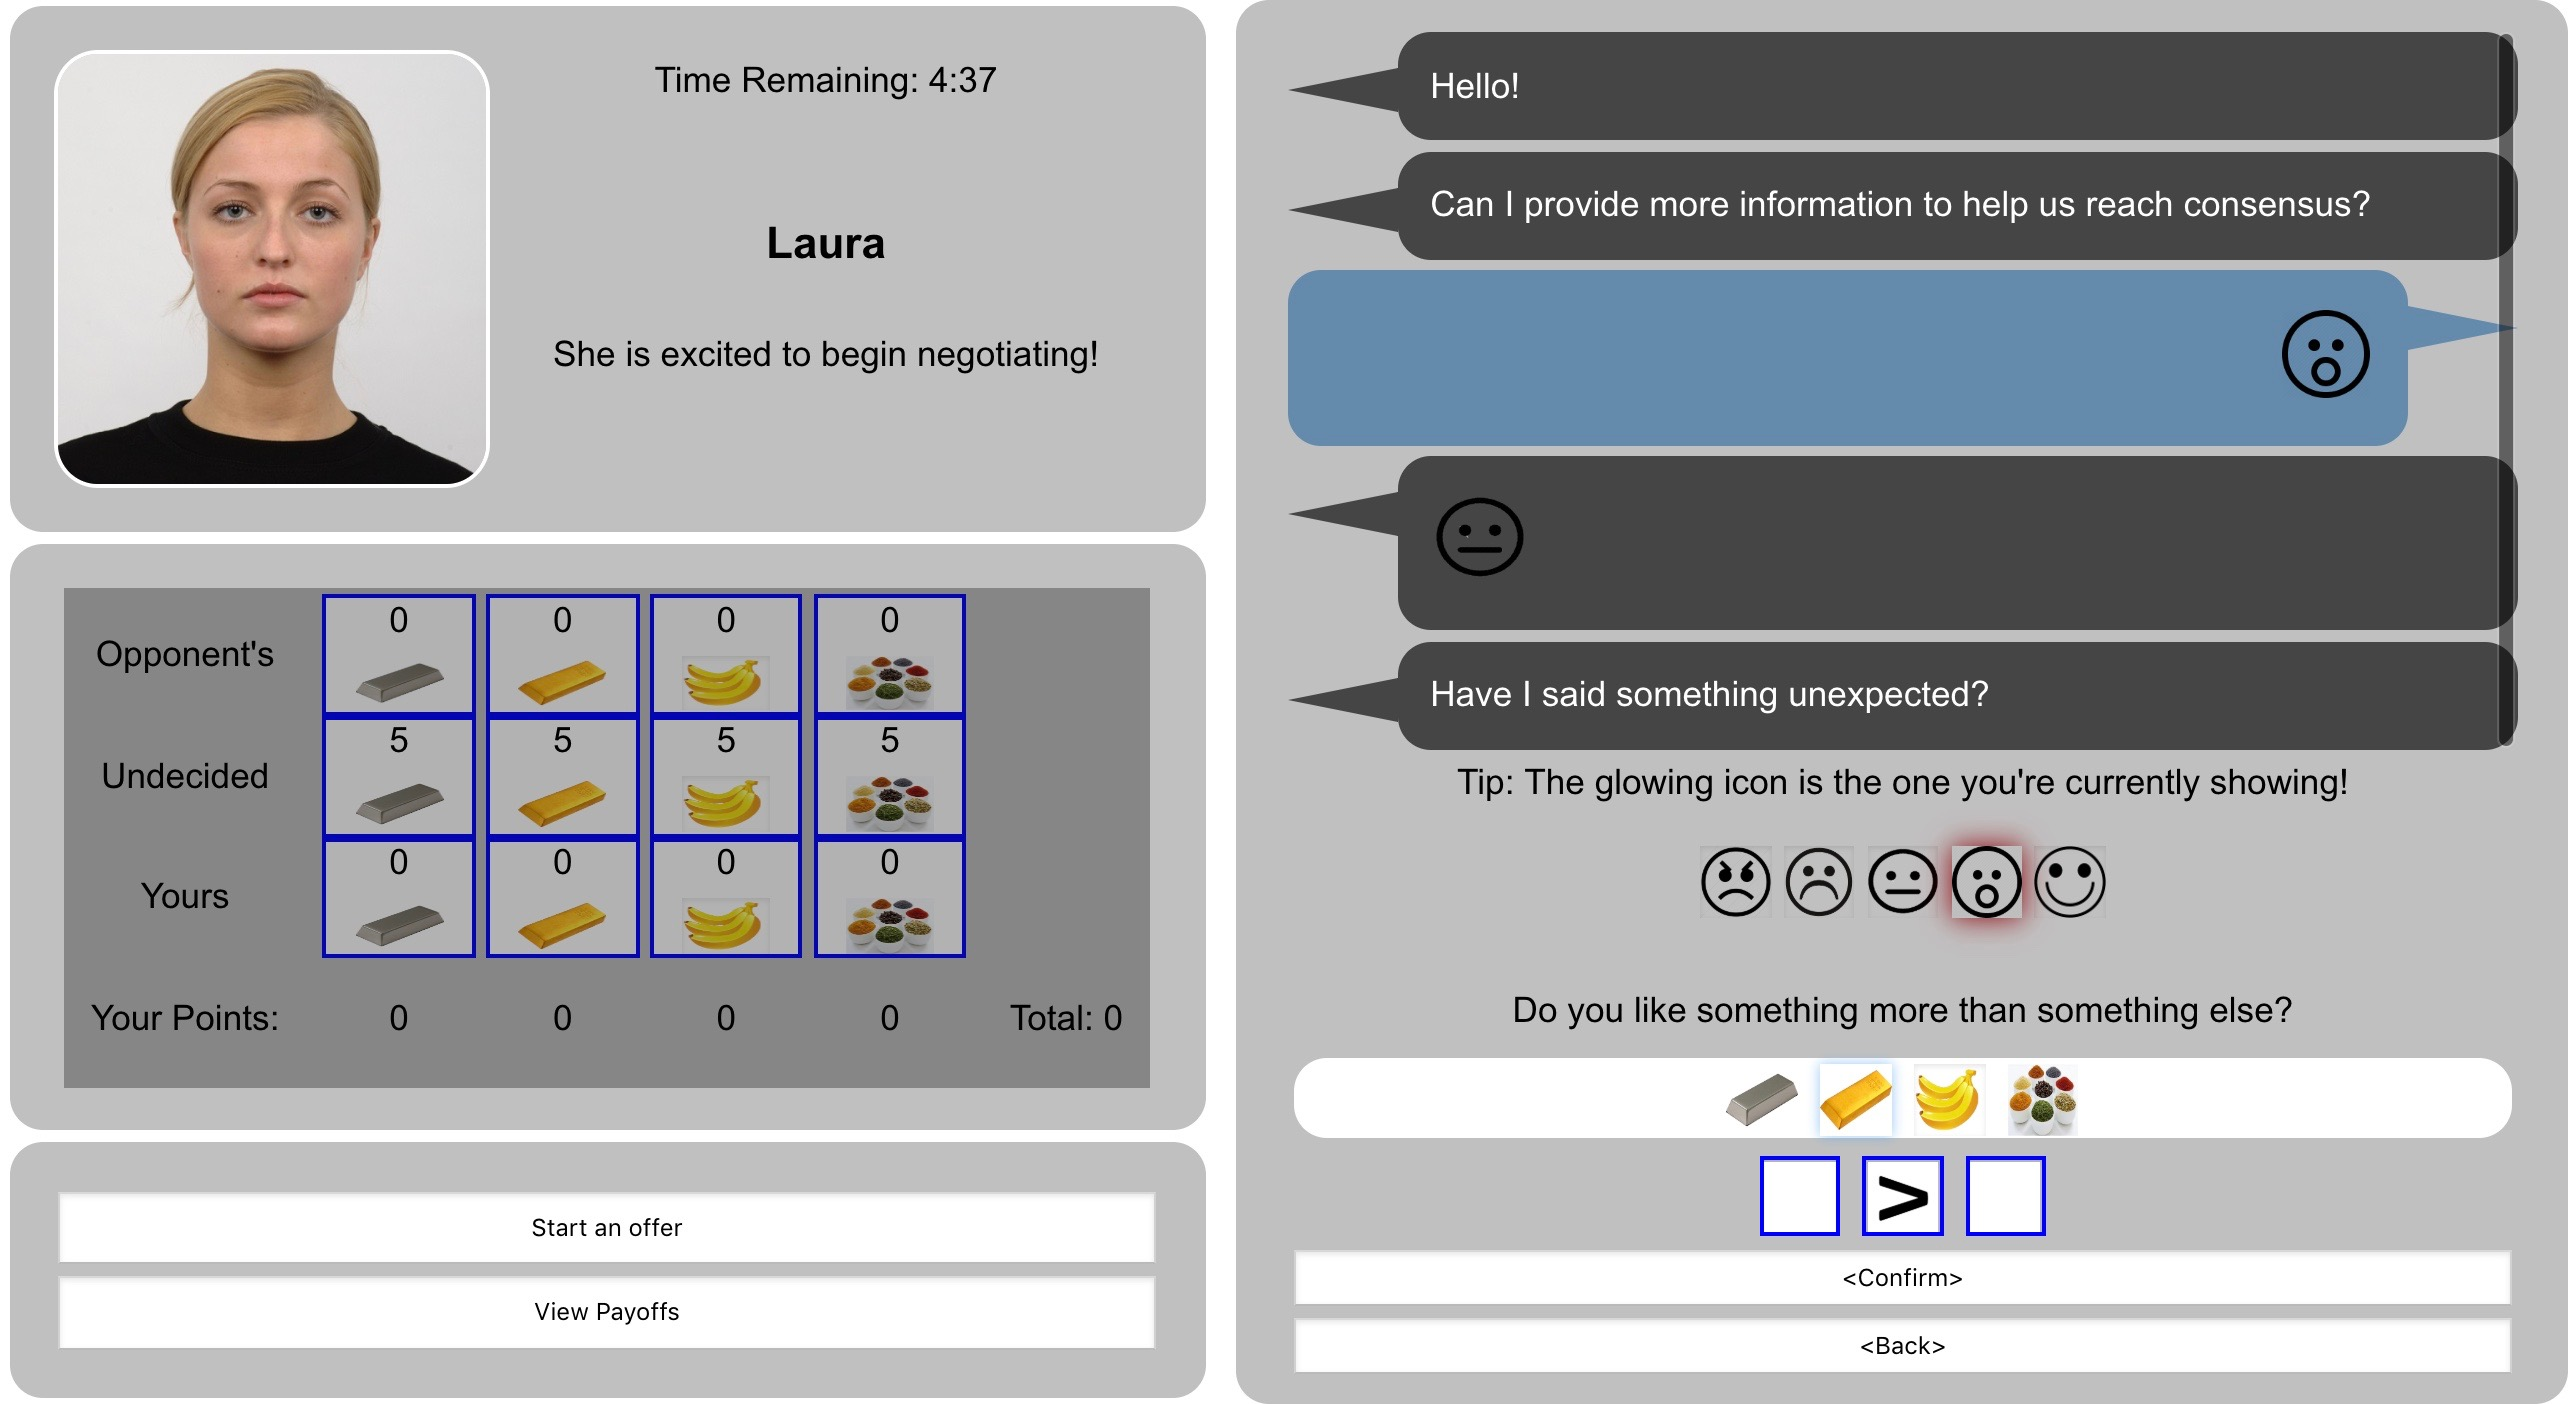
\includegraphics[width=15truecm]{image/IAGO.eps}
  \caption{IAGOのインタフェース}
  \label{fig:iago}
\end{figure}

\subsection{IAGO}
IAGO(Interactive Arbitration Guide Online)はANACのHuman-Agent Negotiationリーグで使用される自動交渉のプラットフォームである\cite{iago}.
IAGOのインタフェースを図\ref{fig:iago}に示す.
IAGOでは,人間と交渉を行うエージェントおよび交渉のドメインを作成することが可能である.IAGOの特徴として以下の3点が挙げられる\cite{pinocchio}.

\begin{enumerate}
  \item WEB上で動作する
  \item APIが公開されている
  \item 人間同士の交渉で用いられるチャネルが利用可能
\end{enumerate}

第1の特徴により,エージェントと交渉を行うクライアントはWEBブラウザ上で交渉を行うことが可能である.
したがって,クライアントはソフトウェアのインストールなどを行うことなく交渉を開始することができる.
第2の特徴により,競技会や研究のためのエージェントおよび交渉ドメインの設計を容易に行うことが可能となる.
第3の特徴により,エージェントおよびクライアントは感情の表出,メッセージの送信,選好の公開および誘発などを交渉中に行うことが可能となる.
これにより,人間同士の交渉で用いられるチャネルによる交渉結果への影響を研究することおよび
これらのチャネルを利用した交渉を行うエージェントを作成することが容易となる.
IAGOでは,サンプルとしてPinocchioエージェントがあらかじめ用意されており,本研究では,Pinocchioエージェントをベースにして戦略の実装し,実験を行う.

\section{自動交渉における心理的効果に関する研究}
人間とエージェントの交渉における心理的効果に関する研究としてCelsoらの研究がある\cite{emotion}.
この研究では,交渉相手がエージェントだと知らされた上で感情が交渉に対して影響を与えるか調査している.
同時に,感情の伝達方法によって交渉に与える効果の差異についても調査している.
交渉はAlternating Offers Protocol\cite{aop}を用いて行い,感情は怒り,喜び,中立の3種類,感情の伝達方法は言語,画像の2種類について実験を行なっている.
実験は150人の被験者に対して行われ,実験の結果,エージェントが怒りの感情を相手に伝えた場合被験者は大きく譲歩し,喜びの感情を相手に伝えた場合被験者はあまり譲歩しないという結果となった.また,感情の伝達方法については譲歩の度合いに有意差はなく,感情は伝達方法とは独立に交渉結果に影響を与え,感情によって交渉結果が異なることが明らかになった.
この研究では,今後の展望として繰り返し交渉において感情のような心理的効果が与える影響について調査する必要性について述べられている.

%内容ここまで

\chapter*{謝辞}
本論文を執筆するにあたり,多数の方々からご指導・ご協力いただきましたことを,心より御礼申し上げます.

指導教員である藤田桂英准教授には,研究の機会を与えていただき,研究の方針に関する助言や発表練習等の
多大なるご指導や助言をいただきましたことを深く感謝いたします.

研究に関する知識のご教示に加えて,本実験の準備を行うにあたってWEBサーバを構築する際にお力添えいただいた松根鷹生様に深く感謝申し上げます.
また,藤田桂英研究室の皆様には研究に必要な知識や意見等をいただいたことを心より感謝いたします.

本実験を行うにあたってお忙しい中ご協力いただいた同期の編入生の方々,および安井貴規様がいなければ本論文は完成に至りませんでした.
心より御礼申し上げます.

最後に,様々な面で私を支えていただいた家族に,心より感謝いたします.ありがとうございました.

\bibliographystyle{plain}
\bibliography{reference}


\begin{comment}
%付録で発表論文をつけてアピールだ!!

\renewcommand{\bibname}{付録 発表論文一覧}
%\chapter{発表論文一覧}

\begin{thebibliography}{99}
\item S. Kakimoto and K. Fujita. 二者間複数論点交渉問題におけるパレートフロント推定手法の提案. Joint Agent Workshop and Symposium, 2014.
\item S. Kakimoto and K. Fujita. Estimating Pareto Fronts using Interdependency between Issues for Bilateral Multi-issue Closed Nonlinear Negotiations. Applications Knowledge and Service Technology for Life, Environment, and Sustainability workshop(KASTLES),2014.
\item S. Kakimoto and K. Fujita. 二者間非線形交渉問題におけるパレートフロント推定を利用した自動交渉エージェントの設計と評価. 情報処理学会 第177回 知能システム研究会, 2014.

\end{thebibliography}

\end{comment}

\end{document}

